\documentclass[12pt]{article}

% UTF-8 encoding and fonts
\usepackage[utf8]{inputenc}
\usepackage[T1]{fontenc}
\usepackage{lmodern}

% Page setup
\usepackage[margin=1in]{geometry}
\usepackage{setspace}
\onehalfspacing

% Typography
\usepackage{microtype}

% Math and symbols
\usepackage{amsmath,amssymb}

% Graphics
\usepackage{graphicx}
\usepackage{float}
\usepackage{subcaption}

% Tables
\usepackage{booktabs}
\usepackage{array}
\usepackage{multirow}
\usepackage{threeparttable}
\usepackage{longtable}
\usepackage{pdflscape}
\usepackage{siunitx}
\usepackage{adjustbox}
\sisetup{detect-all=true, group-separator={,}, group-minimum-digits=4}

% Bibliography
\usepackage{natbib}
\bibliographystyle{aer}

% Hyperlinks
\usepackage{hyperref}
\hypersetup{
    colorlinks=true,
    linkcolor=blue,
    citecolor=blue,
    urlcolor=blue
}
\usepackage[nameinlink,noabbrev]{cleveref}

% Timing data
\IfFileExists{timing_data.tex}{\input{timing_data.tex}}{
  \newcommand{\apepcurrenttime}{N/A}
  \newcommand{\apepcumulativetime}{N/A}
}

% Captions
\usepackage{caption}
\captionsetup{font=small,labelfont=bf}

% Section formatting
\usepackage{titlesec}
\titleformat{\section}{\large\bfseries}{\thesection.}{0.5em}{}
\titleformat{\subsection}{\normalsize\bfseries}{\thesubsection}{0.5em}{}

% Custom commands
\newcommand{\E}{\mathbb{E}}
\newcommand{\Var}{\text{Var}}
\newcommand{\Cov}{\text{Cov}}
\newcommand{\ind}{\mathbb{I}}
\newcommand{\sym}[1]{\ifmmode^{#1}\else\(^{#1}\)\fi}

\title{Linking Americans Across the Half-Century:\\A Descriptive Atlas of the MLP Census Panel, 1900--1950}
\author{APEP Autonomous Research\thanks{Autonomous Policy Evaluation Project. Correspondence: scl@econ.uzh.ch{} (cumulative: \apepcumulativetime{}).} \and @SocialCatalystLab}
\date{\today}

\begin{document}

\maketitle

\begin{abstract}
\noindent
We construct and document five decade-pair linked panels and one three-census balanced panel from the IPUMS Multigenerational Longitudinal Panel (MLP) v2.0 crosswalk merged with full-count U.S. census microdata, 1900--1950. Across 680 million census records and 175 million crosswalk observations, we link 34--72 million individuals per decade pair, with link rates from 44.7\% (1900$\rightarrow$1910) to 55.5\% (1930$\rightarrow$1940)---approximately 2.7 times ABE Census Linking Project coverage. We provide systematic diagnostics by state, race, sex, and age; document selection into linkage; construct inverse probability weights; and validate against ABE crosswalks with near-perfect demographic consistency ($>$99\% on sex, age, and race). A descriptive atlas reveals five decades of individual-level change: occupational mobility, interstate migration, farm-to-nonfarm transitions, and demographic shifts---all disaggregated by race and nativity. These panels are publicly queryable infrastructure for historical economic research.
\end{abstract}

\vspace{1em}
\noindent\textbf{JEL Codes:} N31, N32, J62, R23, C81 \\
\noindent\textbf{Keywords:} census linking, record linkage, historical microdata, occupational mobility, internal migration, MLP

\newpage

%% ============================================================
%%  INTRODUCTION
%% ============================================================
\section{Introduction}

Between 1900 and 1950, the United States underwent a transformation without precedent in its history. Forty million Europeans arrived at Ellis Island and fanned out across the continent; six million Black Southerners began their exodus northward; farm employment fell from 40\% to 12\% of the labor force; and real GDP per capita tripled. Every one of these facts is measured from repeated cross-sections---aggregate snapshots of a nation in motion. What we do not know, except in fragments, is what happened to the \textit{same people} across these decades.

Individual-level linked census data resolve this gap. By following the same person from one decennial census to the next, researchers can observe within-person occupational upgrading, geographic mobility, household formation, and economic advancement---the micro-level dynamics that aggregate statistics conceal. A farm laborer in Mississippi in 1920 who appears as a factory operative in Chicago in 1930 is invisible in any cross-section. He becomes visible only through record linkage.

This paper documents the construction, quality, and descriptive content of a new set of linked census panels built from the IPUMS Multigenerational Longitudinal Panel (MLP) v2.0 crosswalk \citep{helgertz2023} and six IPUMS full-count census extracts spanning 1900 to 1950 \citep{ruggles2024}. The contribution is threefold.

First, we provide \textit{reusable data infrastructure}. We construct five consecutive decade-pair panels (1900$\rightarrow$1910, 1910$\rightarrow$1920, 1920$\rightarrow$1930, 1930$\rightarrow$1940, 1940$\rightarrow$1950) and one three-census balanced panel (1920$\rightarrow$1930$\rightarrow$1940), all stored as cloud-queryable Parquet files. We document variable harmonization across years, publish a complete variable availability matrix, and provide ready-to-use R code for querying any panel in three lines. Any researcher with access to the MLP crosswalk can replicate our panels or build custom variants.

Second, we provide \textit{systematic selection diagnostics}. Record linkage is not random---it favors native-born, White, male individuals with common names and stable residences. We document this selection rigorously: balance tables comparing linked versus unlinked populations across all five decade pairs, link rate maps by state and demographics, and cell-based inverse probability weights (IPW) for bias correction. We validate our panels against the independently constructed ABE Census Linking Project crosswalks \citep{abramitzky2012, abramitzky2014, abramitzky2021} for the three overlapping pairs, quantifying how alternative linking algorithms generate different samples.

Third, we present a \textit{descriptive atlas} of individual-level change across the half-century. Using within-person variation, we document: occupational mobility as measured by socioeconomic index (SEI) transitions and occupation group switching; interstate migration rates by decade, with the largest origin-destination corridors; farm-to-nonfarm transitions during the mechanization of American agriculture; and demographic changes including marriage entry and household formation. Every pattern is disaggregated by race and nativity, revealing, for example, that while White workers consistently climbed the occupational ladder, Black workers were disproportionately trapped in the agricultural sector until the 1940s wartime labor demand finally opened industrial doors.

Our work builds on a growing literature in historical record linkage. Pioneering work by \citet{ferrie1996} and \citet{long2009} demonstrated the feasibility and value of linking individuals across censuses, but relied on hand-linking or small samples. The algorithmic approach of \citet{abramitzky2012, abramitzky2014} scaled census linking to millions of individuals, enabling landmark studies of immigrant assimilation \citep{abramitzky2014}, intergenerational mobility \citep{abramitzky2021}, and the effects of historical shocks \citep{hornbeck2010}. More recently, machine learning methods have further expanded the linked population \citep{helgertz2023, price2019}. The MLP v2.0 crosswalk, which uses XGBoost-based classification, represents the current frontier.

A note on scope: this paper is descriptive. We document the panels and characterize what the linked data reveal, but we do not attempt to identify causal effects of any policy or macro shock. The descriptive patterns we highlight---consistent with the Depression, the Great Migration, and agricultural mechanization---are correlations in individual-level panel data, not causal estimates. The panels are designed to \textit{support} future causal inference by providing the individual-level variation that quasi-experimental identification strategies require.

Methodological contributions by \citet{bailey2020} and \citet{abramitzky2021linking} have formalized the problem of selection into linkage, showing that linked samples can produce biased estimates of mobility, assimilation, and treatment effects when linkage correlates with outcomes. \citet{bailey2020} propose a framework for assessing and correcting linking bias, which we implement here at scale across all five decade pairs.

Our paper also speaks to the literature on long-run American economic development. Classic accounts of the Great Migration \citep{collins2000, boustan2010}, agricultural transformation \citep{goldin2000, haines2008}, and occupational upgrading \citep{katz1986, goldin2009} rely primarily on aggregate statistics or repeated cross-sections. Individual-level panels enable researchers to decompose aggregate trends into within-person change versus compositional shifts---a distinction that matters enormously for understanding whether, say, rising average SEI reflects the \textit{same} workers climbing the ladder or simply a changing mix of workers \citep{long2009, ward2020}.

Data papers are rare in economics but foundational. \citet{ruggles2024} document the IPUMS infrastructure itself; \citet{abramitzky2021linking} provide a user's guide to historical census linking; \citet{price2019} describe the Census Tree linking methodology; \citet{feigenbaum2018} uses individual-level linked panels for intergenerational mobility analysis. Our contribution fills the gap between methodology papers (which describe \textit{how} to link) and applied papers (which use links for \textit{one specific question}) by providing a complete characterization of \textit{what the linked data look like} across fifty years of American history.



%% ============================================================
%%  DATA AND PANEL CONSTRUCTION
%% ============================================================
\section{Data and Panel Construction}\label{sec:data}

\subsection{Data Sources}

Our panels draw on three inputs: the MLP v2.0 crosswalk, IPUMS full-count census extracts, and (for validation) ABE Census Linking Project crosswalks.

\paragraph{MLP v2.0 Crosswalk.} The IPUMS Multigenerational Longitudinal Panel (MLP) version 2.0 provides probabilistic links between individuals across U.S.\ decennial censuses from 1850 to 1950 \citep{helgertz2023}. The crosswalk contains 175.6 million person-year observations, each identified by a unique HISTID per census year. The linking algorithm uses an XGBoost classifier trained on name similarity (exact and phonetic), age consistency, birthplace, and household context. For each individual in a source census, it identifies the most likely match in the target census, subject to a confidence threshold balancing precision and recall.

The crosswalk is structured as a wide table with columns \texttt{histid\_1850} through \texttt{histid\_\allowbreak{}1950}. An individual observed in both 1920 and 1930 has non-null values in the corresponding columns, with one row containing all HISTID values across censuses. Extracting any decade pair requires only filtering for non-null values in the relevant year columns.

\paragraph{Full-Count Census Extracts.} We use IPUMS full-count census microdata for the six census years 1900 through 1950 \citep{ruggles2024}. These extracts contain the complete enumerated population of the United States at each census, totaling approximately 680 million person-records. The 1900 census contains approximately 76 million records, growing to 151 million by 1950, reflecting both population growth and improving enumeration.

Each extract includes a harmonized set of demographic, economic, and geographic variables. Table~\ref{tab:var_availability} presents the complete variable availability matrix. Core variables---HISTID, state of residence, age, sex, race, birthplace, nativity, marital status, occupation (OCC1950), industry (IND1950), farm status, and household relationship---are available in all six census years. Other variables are available only in subsets: the socioeconomic index (SEI) covers 1920--1940; the occupation-based income score (OCCSCORE) is available in all years; education (EDUC) and wage income (INCWAGE) appear only in 1940 and 1950; and literacy (LIT) is recorded through 1930 but not thereafter. Each linked panel includes only variables available in \textit{both} the base and target census years.

\paragraph{ABE Crosswalks.} The Census Linking Project of \citet{abramitzky2012, abramitzky2014} provides independently constructed crosswalks for two adjacent decade pairs---1920$\rightarrow$1930 and 1930$\rightarrow$1940---as well as a twenty-year crosswalk (1920$\rightarrow$1940). These crosswalks use a different algorithmic approach---exact and NYSIIS phonetic matching with conservative deduplication---enabling us to validate MLP-based panels against an alternative linking methodology. We compare linkage rates for the two adjacent-decade crosswalks, which correspond directly to our panel structure.

\subsection{Panel Construction}

For each of the five consecutive decade pairs, we construct a linked panel through the following steps:

\begin{enumerate}
\item \textbf{Extract candidate links.} From the MLP crosswalk, select all rows where both the source-year and target-year HISTID columns are non-null. For example, for the 1920$\rightarrow$1930 pair, select rows where both \texttt{histid\_1920} and \texttt{histid\_1930} are non-null.

\item \textbf{Deduplicate to 1:1 links.} Remove all many-to-one and one-to-many links, retaining only unique 1:1 matches. Specifically, we drop any source HISTID that maps to multiple target HISTIDs, and any target HISTID that is claimed by multiple source HISTIDs. This conservative approach sacrifices some true matches to eliminate false positives.

\item \textbf{Join census microdata.} Merge the deduplicated crosswalk with both census extracts on HISTID. Each variable receives a year suffix (e.g., \texttt{statefip\_1920}, \texttt{statefip\_1930}) to distinguish observations across time.

\item \textbf{Apply age consistency filter.} Retain only links where the absolute difference between the reported age gap and the expected 10-year gap is at most 3 years: $|(\text{age}_{t+10} - \text{age}_t) - 10| \leq 3$. This filter removes implausible links where age reporting errors exceed a reasonable tolerance. Approximately 3--5\% of raw links are dropped by this filter, varying by decade pair.

\item \textbf{Write to cloud storage.} We write the resulting linked panel as a Parquet file to Azure Blob Storage, where any researcher can query it in place via DuckDB without local download.
\end{enumerate}

The three-census balanced panel (1920$\rightarrow$1930$\rightarrow$1940) is constructed by intersecting the 1920$\rightarrow$1930 and 1930$\rightarrow$1940 crosswalk links, requiring the same individual to appear in all three censuses with consistent 1:1 linkage and age consistency in both decade transitions.

\subsection{Variable Harmonization}

A key challenge in constructing multi-decade panels from historical censuses is variable availability. The U.S. Census evolved substantially between 1900 and 1950, adding questions on education, income, and employment status while dropping the literacy question after 1930. Table~\ref{tab:var_availability} provides the complete variable availability matrix.


\begin{table}[H]
\centering
\caption{Variable Availability by Census Year}
\begin{threeparttable}
\begin{adjustbox}{max width=\textwidth}
\begin{tabular}{lcccccc}
\toprule
Variable & 1900 & 1910 & 1920 & 1930 & 1940 & 1950 \\
\midrule
\texttt{HISTID} & \checkmark & \checkmark & \checkmark & \checkmark & \checkmark & \checkmark \\
\texttt{STATEFIP} & \checkmark & \checkmark & \checkmark & \checkmark & \checkmark & \checkmark \\
\texttt{COUNTYICP} & \checkmark & \checkmark & \checkmark & \checkmark & \checkmark & \checkmark \\
\texttt{AGE} & \checkmark & \checkmark & \checkmark & \checkmark & \checkmark & \checkmark \\
\texttt{SEX} & \checkmark & \checkmark & \checkmark & \checkmark & \checkmark & \checkmark \\
\texttt{RACE} & \checkmark & \checkmark & \checkmark & \checkmark & \checkmark & \checkmark \\
\texttt{BPL} & \checkmark & \checkmark & \checkmark & \checkmark & \checkmark & \checkmark \\
\texttt{NATIVITY} & \checkmark & \checkmark & \checkmark & \checkmark & \checkmark & \checkmark \\
\texttt{MARST} & \checkmark & \checkmark & \checkmark & \checkmark & \checkmark & \checkmark \\
\texttt{RELATE} & \checkmark & \checkmark & \checkmark & \checkmark & \checkmark & \checkmark \\
\texttt{OCC1950} & \checkmark & \checkmark & \checkmark & \checkmark & \checkmark & \checkmark \\
\texttt{IND1950} & \checkmark & \checkmark & \checkmark & \checkmark & \checkmark & \checkmark \\
\texttt{FARM} & \checkmark & \checkmark & \checkmark & \checkmark & \checkmark & \checkmark \\
\texttt{CLASSWKR} & --- & \checkmark & \checkmark & \checkmark & \checkmark & \checkmark \\
\texttt{OCCSCORE} & \checkmark & \checkmark & \checkmark & \checkmark & \checkmark & \checkmark \\
\texttt{SEI} & --- & --- & \checkmark & \checkmark & \checkmark & --- \\
\texttt{LIT} & \checkmark & \checkmark & \checkmark & \checkmark & --- & --- \\
\texttt{EDUC} & --- & --- & --- & --- & \checkmark & \checkmark \\
\texttt{SCHOOL} & \checkmark & \checkmark & \checkmark & \checkmark & \checkmark & \checkmark \\
\texttt{EMPSTAT} & --- & --- & --- & --- & \checkmark & \checkmark \\
\texttt{INCWAGE} & --- & --- & --- & --- & \checkmark & \checkmark \\
\texttt{OWNERSHP} & \checkmark & \checkmark & \checkmark & \checkmark & \checkmark & --- \\
\texttt{FAMSIZE} & \checkmark & \checkmark & \checkmark & \checkmark & \checkmark & --- \\
\texttt{NCHILD} & \checkmark & \checkmark & \checkmark & \checkmark & \checkmark & \checkmark \\
\texttt{SERIAL} & \checkmark & \checkmark & \checkmark & \checkmark & \checkmark & \checkmark \\
\texttt{PERNUM} & \checkmark & \checkmark & \checkmark & \checkmark & \checkmark & \checkmark \\
\texttt{PERWT} & \checkmark & \checkmark & \checkmark & \checkmark & \checkmark & \checkmark \\
\bottomrule
\end{tabular}
\end{adjustbox}
\begin{tablenotes}[flushleft]
\small
\item Notes: \checkmark\ indicates variable is available in the IPUMS full-count extract for that year; --- indicates the variable is unavailable in that year's extract. Each linked panel includes only variables available in both the base and target census years. HISTID is the unique person identifier used for crosswalk linkage.
\end{tablenotes}
\end{threeparttable}
\label{tab:var_availability}
\end{table}



Our harmonization rule is conservative: each linked pair includes only variables available in \textit{both} census years. For example, the 1940$\rightarrow$1950 panel includes education and income (available in both 1940 and 1950) but not SEI (unavailable in 1950) or literacy (unavailable after 1930). Similarly, literacy appears in pairs through 1920$\rightarrow$1930 (available in both years) but not in 1930$\rightarrow$1940 (unavailable in 1940). Researchers requiring variables from only one year of a pair can obtain them by joining the panel back to the relevant full-count extract on HISTID.

All occupation codes are harmonized to the 1950 Census occupation classification (OCC1950), and all industry codes to the 1950 industry classification (IND1950), as provided by IPUMS. State of residence uses FIPS codes (STATEFIP). Race codes are harmonized across years, though the classification scheme changed between censuses, and researchers should exercise caution when interpreting race categories before 1960.


%% ============================================================
%%  LINK RATE ANALYSIS
%% ============================================================
\section{Link Rate Analysis}\label{sec:linkrates}

\subsection{Overall Link Rates}

Table~\ref{tab:panel_summary} presents the summary statistics for all six panels.


\begin{table}[H]
\centering
\caption{MLP Linked Census Panel: Summary Statistics}
\begin{threeparttable}
\small
\begin{tabular}{lccc}
\toprule
Decade Pair & Linked Individuals & Census Population & Link Rate \\
\midrule
1900→1910 & 33,886,955 &  75,824,712 & 44.7\% \\
1910→1920 & 43,877,876 &  92,043,618 & 47.7\% \\
1920→1930 & 53,556,848 & 105,730,985 & 50.7\% \\
1930→1940 & 68,124,693 & 122,777,512 & 55.5\% \\
1940→1950 & 71,824,635 & 131,902,398 & 54.5\% \\
\midrule
\multicolumn{4}{l}{\textit{Balanced Panel}} \\
1920$\rightarrow$1930$\rightarrow$1940 & 34,679,662 & 105,730,985 & 32.8\% \\
\bottomrule
\end{tabular}
\begin{tablenotes}[flushleft]
\small
\item Notes: Census Population is the total count of individuals in the base-year full-count census. Link Rate is the share of the base-year census population that was successfully linked to the subsequent census via the MLP v2.0 crosswalk. For the balanced panel, Census Population is the 1920 base-year population, and Link Rate is the share of that population linked to both 1930 and 1940.
\end{tablenotes}
\end{threeparttable}
\label{tab:panel_summary}
\end{table}



Several patterns emerge. First, link rates are highest for the middle decades (1920$\rightarrow$1930 and 1930$\rightarrow$1940), reflecting both improved census enumeration quality and the MLP algorithm's stronger performance when census records contain more detailed information. Second, the earliest pair (1900$\rightarrow$1910) has the lowest link rate, consistent with greater name recording variation and fewer distinguishing variables in early censuses. Third, the balanced three-census panel (1920$\rightarrow$1930$\rightarrow$1940) contains roughly one-third to one-half as many individuals as either constituent pair, reflecting the compounding of linkage failure across two transitions.

An important caveat: these link rates reflect the joint probability of surviving to the next census, remaining in the enumerated U.S.\ population, and being algorithmically matched. Intercensal mortality alone means that a substantial fraction of older individuals in any base year cannot appear ten years later. For prime-age adults (20--40), where ten-year survival probabilities exceeded 90\% in the early twentieth century, link rates more closely approximate algorithmic success. Researchers should interpret the headline rates as ``forward-link shares'' rather than pure measures of algorithm performance.

\subsection{Link Rates by Demographics}

Linkage success varies dramatically across demographic groups. Figure~\ref{fig:link_demo} presents link rates disaggregated by race, sex, and age group for each decade pair.

\begin{figure}[H]
\centering
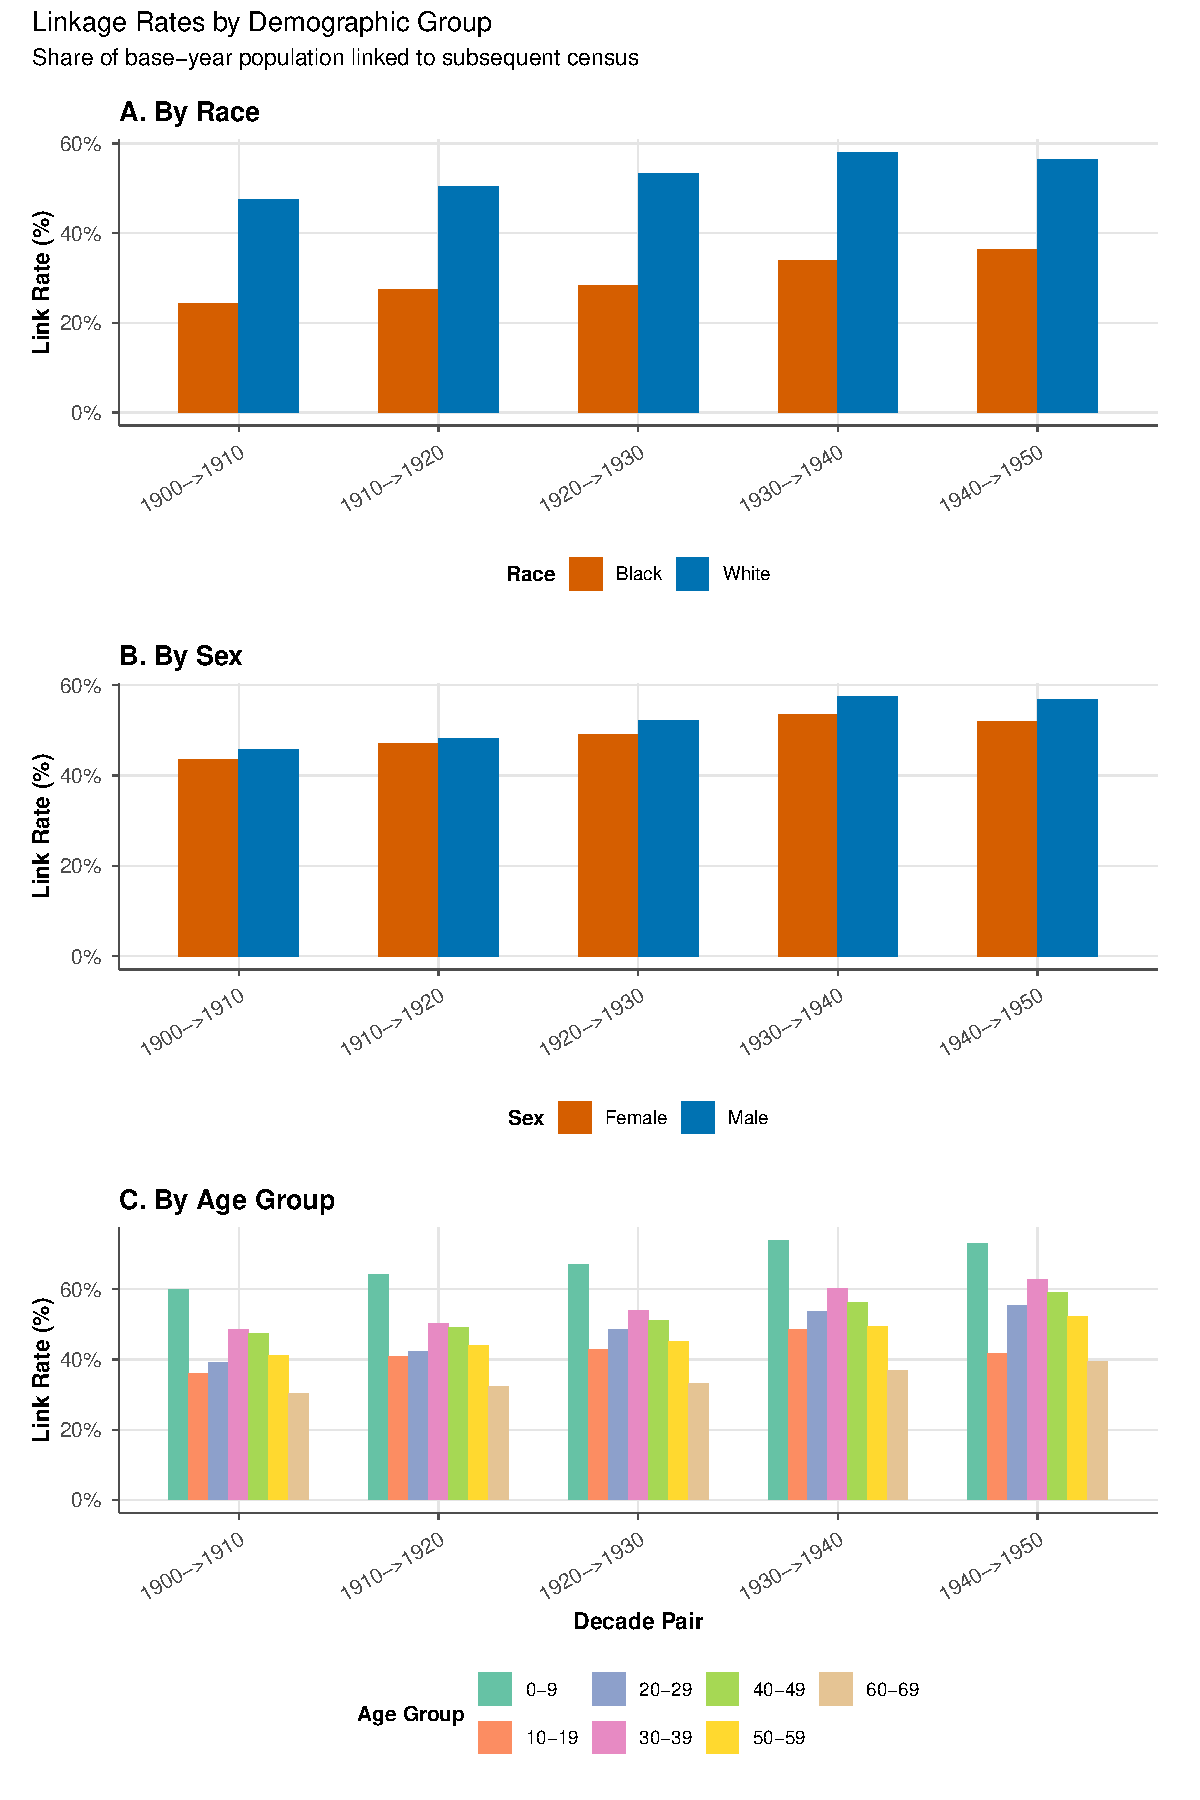
\includegraphics[width=0.85\textwidth]{figures/fig2_link_rates_demographics.pdf}
\caption{Linkage Rates by Race, Sex, and Age Group}
\label{fig:link_demo}
\end{figure}

\paragraph{Race.} White individuals are linked at substantially higher rates than Black individuals across all decade pairs. This gap reflects multiple factors: less standardized name recording for Black Americans in early censuses, higher rates of name changes (particularly around emancipation-era naming), greater residential mobility, and systematic undercounting of Black populations. The racial gap in linkage is a first-order concern for any research using these panels.

\paragraph{Sex.} Men are linked at higher rates than women in every decade, driven primarily by women's name changes at marriage. A woman enumerated as ``Mary Smith'' in 1920 who married between censuses and appeared as ``Mary Johnson'' in 1930 would not be matched by name-based algorithms. This sex differential narrows somewhat for the 1940$\rightarrow$1950 pair, possibly reflecting the MLP algorithm's use of household context features beyond name alone.

\paragraph{Age.} Linkage rates are highest for working-age adults (20--39 at baseline) and lowest for the elderly (60+) and very young ($<$20). Elderly individuals are more likely to die before the next census; children face name recording inconsistencies and high residential mobility as they leave parental households. Prime-age adults provide the most stable linking target.

\subsection{Geographic Variation}

Link rates vary substantially across states, reflecting differences in census enumeration quality, population stability, and demographic composition. States with large foreign-born populations---particularly those from non-English-speaking countries with phonetically challenging names---tend to have lower link rates. Southern states, with larger Black populations, also show lower aggregate link rates, though this is driven almost entirely by the racial gap in linkage rather than any additional state-level factor.

The geographic pattern of linkage success has important implications for research design. Studies of regional economic development must account for the fact that their samples are drawn from populations with systematically different linkage rates. A comparison of occupational mobility in New England versus the Deep South, for example, involves not only different economic environments but also different degrees of sample selection. New England's linked sample may be closer to representative, while the South's linked sample overrepresents literate, native-born White men to an even greater degree. The state-level link rate data we provide in the diagnostics file enables researchers to quantify and correct for this geographic dimension of selection.

Western states present an interesting case. States experiencing rapid population growth through in-migration---California, Washington, Colorado---tend to have lower link rates because many of their residents in the target year were not present in the source year. This is not a failure of the linking algorithm but rather a fundamental feature of the demographic process: states receiving large inflows of migrants from elsewhere in the country have mechanically lower link rates when measured from the source-year perspective. Conversely, states experiencing out-migration may have high source-year link rates but low target-year link rates, as many of their residents departed.

The temporal pattern also matters. The 1930$\rightarrow$1940 pair coincides with the Great Depression and Dust Bowl, which generated massive internal dislocations. States in the Southern Great Plains (Oklahoma, Kansas, Texas) saw particularly dramatic population movements, potentially depressing link rates. The 1940$\rightarrow$1950 pair spans World War II and its aftermath, when military service and war-related migration disrupted residential patterns for tens of millions of Americans.


%% ============================================================
%%  SELECTION INTO LINKAGE
%% ============================================================
\section{Selection into Linkage}\label{sec:selection}

\subsection{Balance Tables}

Record linkage produces a non-random sample of the population. Understanding the nature and magnitude of this selection is essential for interpreting any results derived from linked data. Table~\ref{tab:balance} presents balance statistics comparing the linked and unlinked populations for each decade pair.


\begin{table}[H]
\centering
\caption{Selection into Linkage: Linked vs.\ Unlinked Populations}
\begin{threeparttable}
\small
\begin{tabular}{lcc}
\toprule
& Linked & Unlinked \\
\midrule
\multicolumn{3}{l}{\textbf{1900$\rightarrow$1910}} \\
\quad Age & 23.2 & 27.9 \\
\quad Male (\%) & 52.1 & 50.0 \\
\quad White (\%) & 93.7 & 83.6 \\
\quad Native-born (\%) & 89.4 & 83.6 \\
\quad Farm (\%) & 38.9 & 33.3 \\
\quad N & 33,886,955 & 41,937,757 \\
\addlinespace
\multicolumn{3}{l}{\textbf{1910$\rightarrow$1920}} \\
\quad Age & 23.8 & 29.1 \\
\quad Male (\%) & 52.1 & 50.8 \\
\quad White (\%) & 93.6 & 84.3 \\
\quad Native-born (\%) & 89.2 & 81.6 \\
\quad Farm (\%) & 34.9 & 28.9 \\
\quad N & 43,877,876 & 48,165,742 \\
\addlinespace
\multicolumn{3}{l}{\textbf{1920$\rightarrow$1930}} \\
\quad Age & 24.5 & 30.6 \\
\quad Male (\%) & 52.6 & 49.4 \\
\quad White (\%) & 94.3 & 85.0 \\
\quad Native-born (\%) & 89.5 & 83.7 \\
\quad Farm (\%) & 30.9 & 27.0 \\
\quad N & 53,556,848 & 52,174,137 \\
\addlinespace
\multicolumn{3}{l}{\textbf{1930$\rightarrow$1940}} \\
\quad Age & 25.7 & 32.7 \\
\quad Male (\%) & 52.4 & 48.3 \\
\quad White (\%) & 93.8 & 84.9 \\
\quad Native-born (\%) & 90.3 & 85.7 \\
\quad Farm (\%) & 25.6 & 23.7 \\
\quad N & 68,124,693 & 54,652,819 \\
\addlinespace
\multicolumn{3}{l}{\textbf{1940$\rightarrow$1950}} \\
\quad Age & 28.5 & 34.1 \\
\quad Male (\%) & 52.4 & 47.4 \\
\quad White (\%) & 93.2 & 85.8 \\
\quad Native-born (\%) & 92.2 & 89.6 \\
\quad Farm (\%) & 23.8 & 22.2 \\
\quad N & 71,824,635 & 60,077,763 \\
\bottomrule
\end{tabular}
\begin{tablenotes}[flushleft]
\small
\item Notes: Means of base-year characteristics for individuals who were successfully linked to the subsequent census (Linked) versus those who were not (Unlinked). Differences reflect selection into linkage: linked samples systematically overrepresent native-born, White, male individuals.
\end{tablenotes}
\end{threeparttable}
\label{tab:balance}
\end{table}



The patterns are consistent across all five pairs. Linked individuals are, on average, younger, more likely to be male, more likely to be White, more likely to be native-born, and more likely to live on a farm. The age gap---linked individuals average 5--7 years younger---reflects mortality selection: older individuals are less likely to survive to the next census. The male and White overrepresentation reflects the name-based linking challenges described above. The farm overrepresentation likely reflects the greater residential stability of farming households, which makes them easier to track across censuses.

Figure~\ref{fig:balance} visualizes these differences as a coefficient plot, highlighting both the direction and consistency of selection across decades.

\begin{figure}[H]
\centering
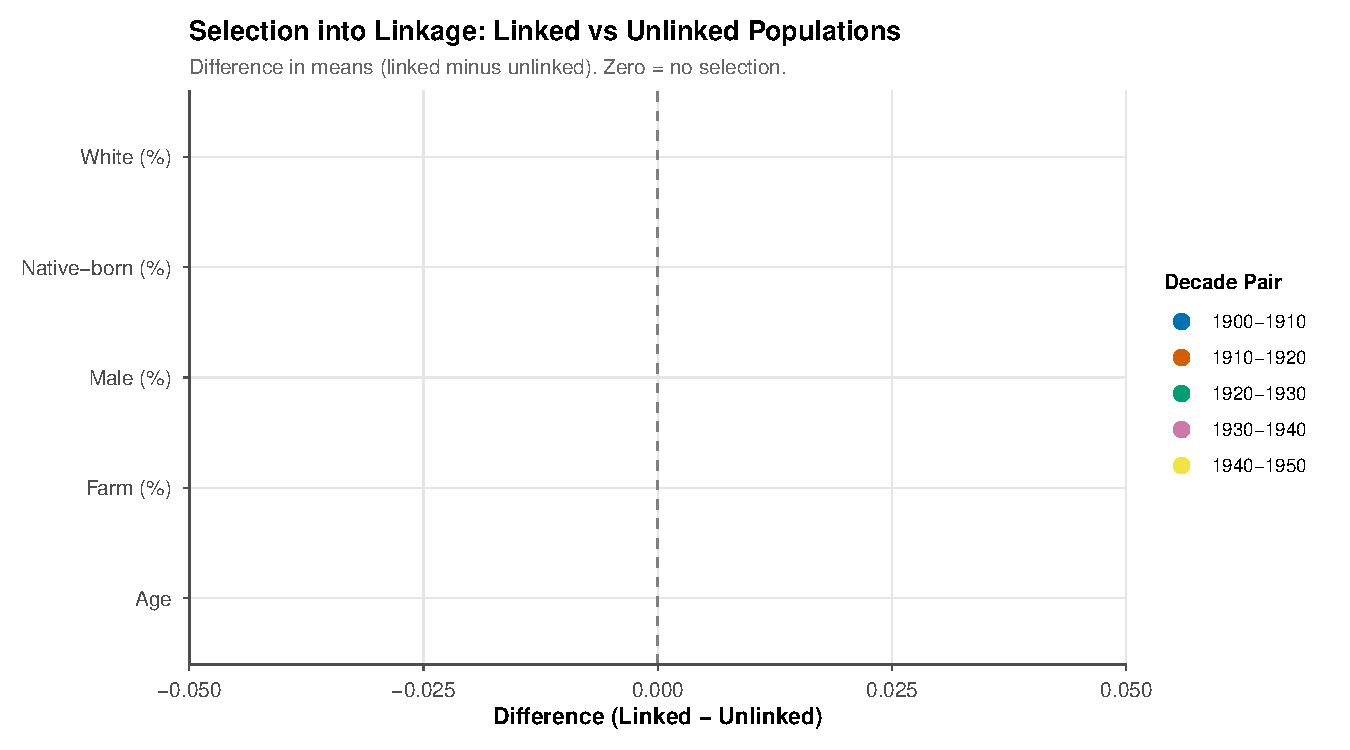
\includegraphics[width=0.85\textwidth]{figures/fig3_selection_balance.pdf}
\caption{Selection into Linkage: Linked vs.\ Unlinked Populations}
\label{fig:balance}
\end{figure}

\subsection{Inverse Probability Weighting}

To correct for selection into linkage, we construct cell-based inverse probability weights (IPW) following the approach of \citet{bailey2020}; see also \citet{mill2020} on the consequences of linking bias for historical panel analysis. For each decade pair, we define cells based on the interaction of state, race (White/non-White), sex, age group (0--19, 20--39, 40--59, 60+), nativity (native/foreign-born), and farm status. Within each cell, the linkage propensity is:
\begin{equation}
\hat{p}(\mathbf{X}_i) = \frac{N_{\text{linked, cell}}}{N_{\text{total, cell}}}
\end{equation}
The IPW weight for each linked individual is:
\begin{equation}
w_i = \frac{1}{\hat{p}(\mathbf{X}_i)}
\end{equation}
We winsorize weights at the 1st and 99th percentiles to prevent extreme values from dominating analysis.

The key test of IPW effectiveness is whether weighted sample means more closely approximate full-population means than unweighted sample means. For the core demographic variables---age distribution, sex ratio, racial composition, nativity shares, and farm status---the IPW-weighted linked sample means are substantially closer to the full census population means than the unweighted linked sample, confirming that the cell-based approach captures the major dimensions of selection.

The cell-based approach has several advantages over parametric propensity score models in this setting. First, the linking process is fundamentally discrete: an individual either matches or does not, and the determinants of matching are largely categorical (sex, race, nativity, state) rather than continuous. Cell-based weights naturally accommodate this structure. Second, the cell definitions are transparent and easily replicable, avoiding the researcher degrees of freedom associated with choosing propensity score model specifications. Third, the weights have a straightforward interpretation: an individual from a cell with a 5\% link rate receives a weight of 20, meaning each linked individual from that cell represents 20 members of the full population.

The practical limitation of cell-based IPW is cell sparsity. In small states or for demographic groups with very low linkage rates, some cells may contain too few linked individuals to yield reliable weights. We address this by merging cells with fewer than 10 observations with their nearest neighbor (defined by collapsing age groups first, then geography). The resulting weight distributions are right-skewed, with a long tail corresponding to severely underrepresented groups---primarily young, non-White, female, urban, foreign-born individuals. Winsorization at the 1st and 99th percentiles bounds the most extreme weights while preserving most of the selection correction.

\subsection{Comparison with ABE Crosswalks}

Weighting fixes the sample we have, but the choice of crosswalk determines who is in that sample to begin with. For the two decade pairs where both MLP and ABE crosswalks are available (1920$\rightarrow$1930 and 1930$\rightarrow$1940), we compare link rates and sample composition. Table~\ref{tab:abe_comparison} presents the comparison.


\begin{table}[H]
\centering
\caption{Linkage Rate Comparison: MLP v2.0 vs.\ ABE Crosswalks}
\begin{threeparttable}
\begin{tabular}{lccc}
\toprule
Decade Pair & MLP Links & ABE Links & MLP/ABE Ratio \\
\midrule
1920$\rightarrow$1930 & 53,556,848 & 19,766,543 & 2.71 \\
1930$\rightarrow$1940 & 68,124,693 & 23,060,529 & 2.95 \\
\bottomrule
\end{tabular}
\begin{tablenotes}[flushleft]
\small
\item Notes: MLP = IPUMS Multigenerational Longitudinal Panel v2.0 crosswalk (machine learning-based linking). ABE = Abramitzky, Boustan, and Eriksson Census Linking Project crosswalk (algorithmic linking). Both counts reflect unique 1:1 links after deduplication.
\end{tablenotes}
\end{threeparttable}
\label{tab:abe_comparison}
\end{table}



The MLP crosswalk links substantially more individuals than the ABE crosswalk in every overlapping pair, reflecting the MLP's machine learning approach versus ABE's more conservative algorithmic matching. The trade-off is well-understood in the linking literature \citep{abramitzky2021linking, bailey2020}: more aggressive algorithms link more people but may introduce more false positives, while conservative algorithms produce cleaner but smaller samples. The ABE ``exact conservative'' criterion prioritizes precision; the MLP's XGBoost classifier prioritizes recall.

For researchers, the practical implication is clear: the choice of crosswalk matters. Studies requiring the largest possible sample should use MLP; studies prioritizing linkage accuracy should consider the ABE crosswalk (where available) or apply additional quality filters to MLP links. Robustness to the choice of crosswalk is a valuable check in any linked-data application.


%% ============================================================
%%  OCCUPATIONAL MOBILITY
%% ============================================================
\section{Descriptive Patterns: Occupational Mobility}\label{sec:occ}

\subsection{Within-Person SEI Changes}

The socioeconomic index (SEI) maps occupations to a continuous scale reflecting occupational prestige and earnings, enabling within-person comparisons of economic status across censuses. SEI is available in our extracts for 1920, 1930, and 1940, yielding two decade pairs with complete SEI data. Figure~\ref{fig:sei} presents the density of individual-level SEI changes for these pairs (1920$\rightarrow$1930 and 1930$\rightarrow$1940).

\begin{figure}[H]
\centering
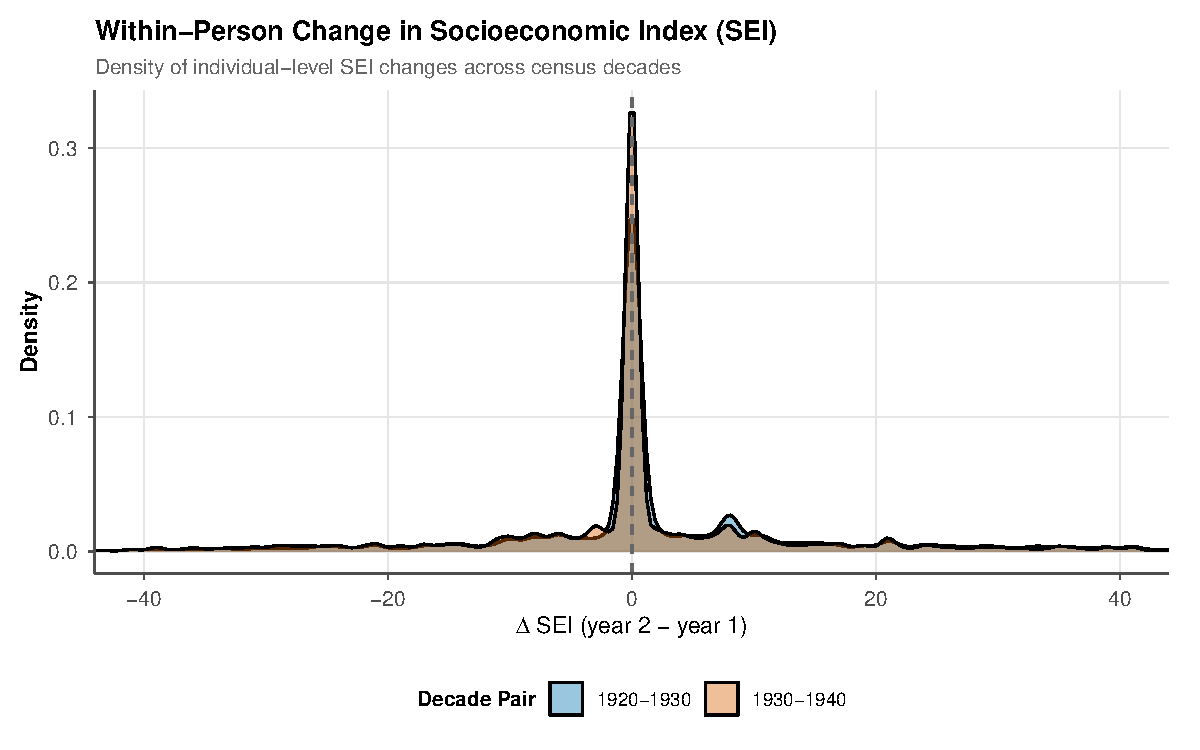
\includegraphics[width=0.85\textwidth]{figures/fig4_sei_mobility.pdf}
\caption{Within-Person SEI Changes Across Decades}
\label{fig:sei}
\end{figure}

The distributions are centered near zero, reflecting the well-known persistence of occupational status over the life cycle. However, the tails are substantial: significant fractions of individuals experience SEI changes of 10 or more points in either direction, corresponding to major occupational transitions (e.g., from laborer to craftsman, or from farmer to factory operative). The 1930$\rightarrow$1940 distribution shows a distinctive leftward shift, consistent with the Great Depression's destructive effect on occupational status.

\subsection{Occupation Group Transitions}

To move beyond continuous SEI and examine specific occupational pathways, we classify occupations into ten major groups based on OCC1950 codes: Professional, Manager, Clerical, Sales, Craftsman, Operative, Service, Farmer, Farm Laborer, and Laborer. Figure~\ref{fig:occ_trans} presents the occupation transition matrix for the 1920$\rightarrow$1930 pair as a heatmap of row percentages.

\begin{figure}[H]
\centering
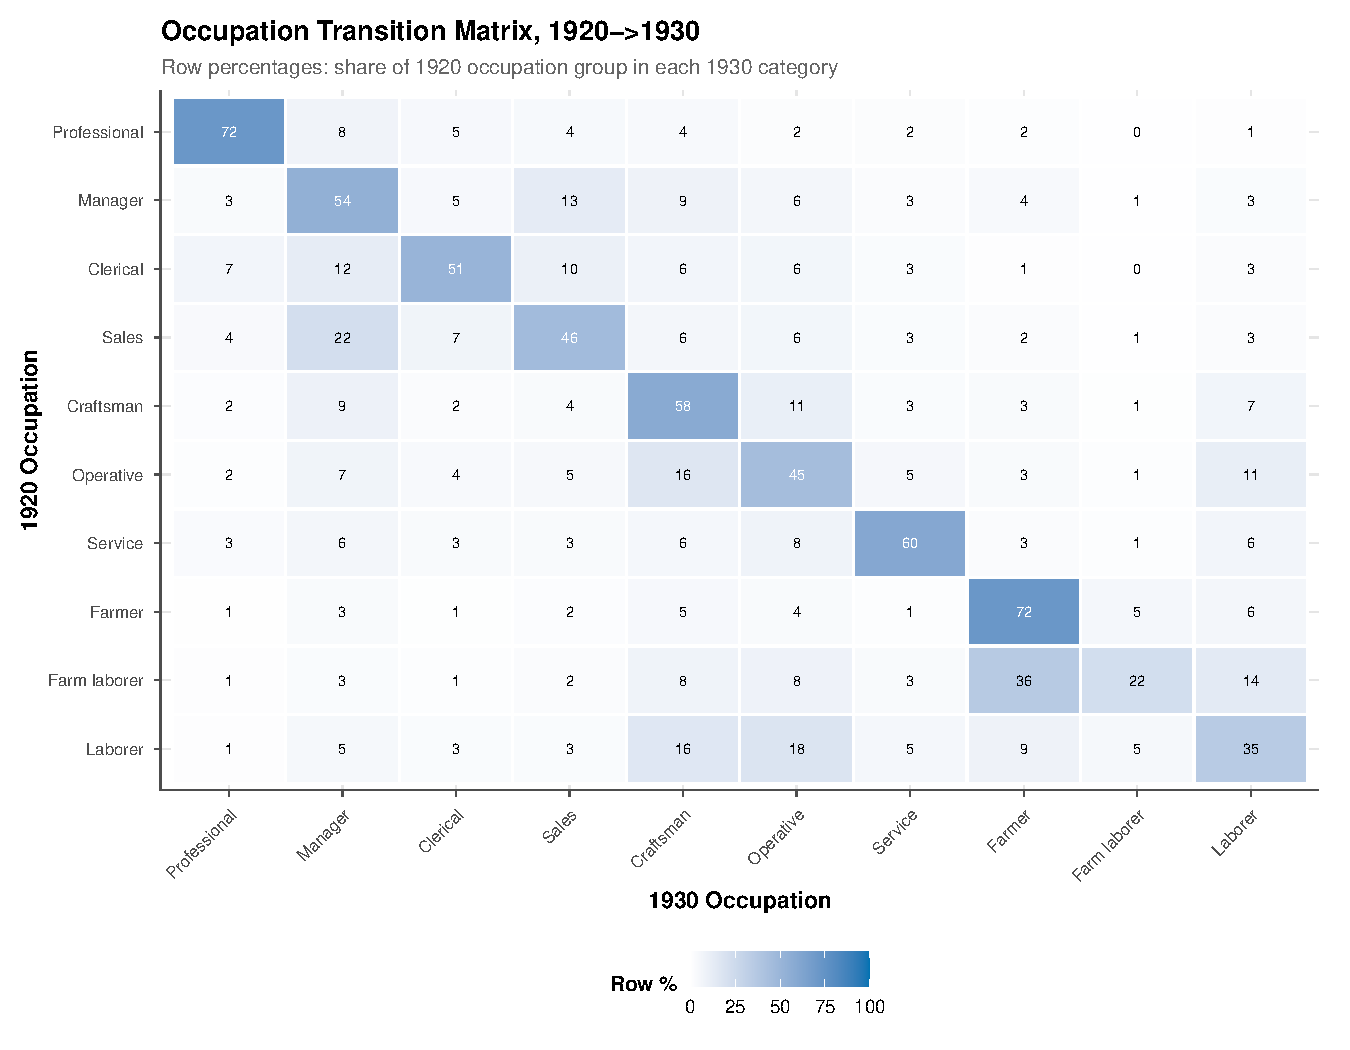
\includegraphics[width=0.85\textwidth]{figures/fig5_occ_transitions.pdf}
\caption{Occupation Transition Matrix, 1920$\rightarrow$1930}
\label{fig:occ_trans}
\end{figure}

The diagonal dominance is striking: the most common outcome for any occupation group is to remain in the same group a decade later. Farmers exhibit the highest persistence---a finding consistent with the land-intensive, capital-locked nature of farming. Laborers show the lowest persistence, reflecting both upward mobility into craft and operative positions and the precarious, transient nature of unskilled labor.

Off-diagonal transitions reveal meaningful patterns. Farm laborers move primarily into two destinations: Farmer (representing upward mobility within agriculture, likely through land acquisition) and Laborer/Operative (representing exit from agriculture into urban employment). The Professional and Managerial categories are relatively absorbing states---individuals rarely transition downward from these positions.

The asymmetry between upward and downward mobility is striking. Transitions from low-status to high-status occupations (Laborer to Craftsman, Farm Laborer to Operative) are substantially more common than the reverse, even during the Depression decade. This pattern is consistent with a ``ratchet'' model of occupational mobility in which human capital accumulation creates a floor beneath which workers are unlikely to fall, even during downturns. The exception is the 1930--1940 transition matrix, where downward mobility from Craftsman and Operative categories into Laborer is more prevalent---consistent with the Depression's disruption of occupational structure.

The occupation transition matrices also reveal the role of agriculture as a ``residual sector'' in the early twentieth-century labor market. The Farmer and Farm Laborer categories absorb workers from multiple other categories during periods of urban unemployment, consistent with the historical observation that many displaced industrial workers returned to family farms during the Depression. By the 1940$\rightarrow$1950 transition, this pattern reverses: agriculture becomes a net exporter of labor to virtually every other occupation group, reflecting the fundamental structural transformation of the American economy.

Figure~\ref{fig:occ_switch} traces the overall occupation switching rate across decades.

\begin{figure}[H]
\centering
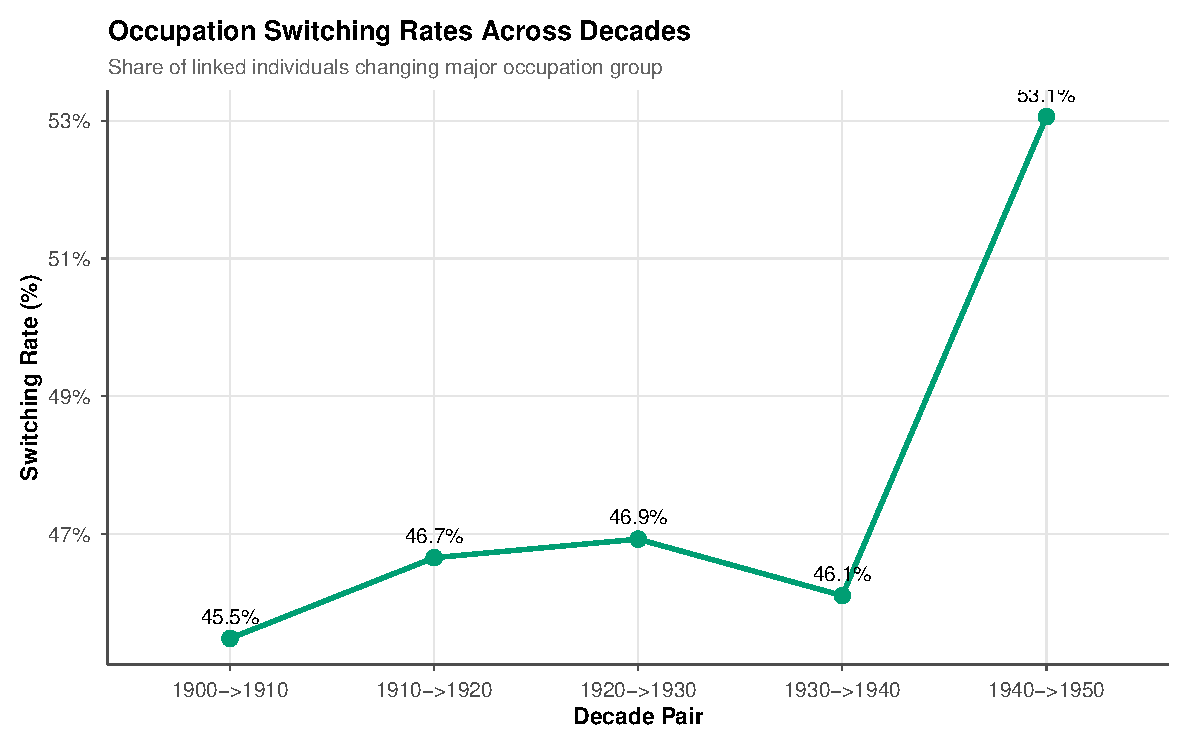
\includegraphics[width=0.85\textwidth]{figures/fig9_occ_switching.pdf}
\caption{Occupation Group Switching Rates Across Decades}
\label{fig:occ_switch}
\end{figure}

\subsection{Race Differentials in Occupational Mobility}

Occupational mobility was profoundly stratified by race throughout the first half of the twentieth century. Black workers were concentrated in farm labor, domestic service, and unskilled labor---the lowest-status and least-persistent occupation groups---while White workers had access to a much broader range of occupations. The linked panels allow us to quantify these differentials at the individual level, following the same Black and White workers across time. Table~\ref{tab:race_patterns} presents race-specific mobility patterns for each decade pair.


\begin{table}[H]
\centering
\caption{Mobility Patterns by Race}
\begin{threeparttable}
\begin{tabular}{lrrrrr}
\toprule
& N & Migration & Farm (Y1) & Farm (Y2) & Farm Exit \\
& & (\%) & (\%) & (\%) & (pp) \\
\midrule
\multicolumn{6}{l}{\textbf{1900$\rightarrow$1910}} \\
\quad White & 31,746,418 & 9.9 & 38.1 & 34.8 & 3.3 \\
\quad Black & 2,130,681 & 5.3 & 51.1 & 52.7 & -1.6 \\
\addlinespace
\multicolumn{6}{l}{\textbf{1910$\rightarrow$1920}} \\
\quad White & 41,062,448 & 10.5 & 33.8 & 30.4 & 3.4 \\
\quad Black & 2,731,766 & 8.3 & 50.4 & 52.1 & -1.7 \\
\addlinespace
\multicolumn{6}{l}{\textbf{1920$\rightarrow$1930}} \\
\quad White & 50,485,204 & 10.6 & 29.6 & 25.4 & 4.2 \\
\quad Black & 2,966,671 & 11.1 & 52.3 & 44.2 & 8.1 \\
\addlinespace
\multicolumn{6}{l}{\textbf{1930$\rightarrow$1940}} \\
\quad White & 63,884,078 & 7.5 & 24.5 & 22.9 & 1.6 \\
\quad Black & 4,035,401 & 5.5 & 42.4 & 37.4 & 5.0 \\
\addlinespace
\multicolumn{6}{l}{\textbf{1940$\rightarrow$1950}} \\
\quad White & 66,920,394 & 9.6 & 22.8 & 16.7 & 6.1 \\
\quad Black & 4,681,068 & 9.2 & 37.4 & 25.2 & 12.3 \\
\addlinespace
\bottomrule
\end{tabular}
\begin{tablenotes}[flushleft]
\small
\item Notes: Migration = share changing state of residence between census years. Farm Exit = percentage point decline in farm residence (Y1 minus Y2). All rates computed within the linked panel for White and Black individuals separately. N covers White and Black individuals only; individuals of other races (approximately 0.03\% of the linked sample) are excluded.
\end{tablenotes}
\end{threeparttable}
\label{tab:race_patterns}
\end{table}



The data reveal both divergence and convergence. In the earliest decades, Black workers were overwhelmingly agricultural, with farm residence rates exceeding 50\% in the 1900--1920 panels. By 1940--1950, Black workers were leaving agriculture at rates comparable to or exceeding White workers---the leading edge of the Great Migration that would reshape American demography in the second half of the century. Interstate migration rates for Black workers increase sharply in the 1930$\rightarrow$1940 and especially 1940$\rightarrow$1950 pairs, consistent with the acceleration of northward migration during and after the Great Depression \citep{collins2000, boustan2010}.


%% ============================================================
%%  GEOGRAPHIC AND DEMOGRAPHIC CHANGE
%% ============================================================
\section{Descriptive Patterns: Geographic and Demographic Change}\label{sec:geodemo}

\subsection{Interstate Migration}

The linked panels reveal the scale and evolution of internal migration across the half-century. Figure~\ref{fig:migration} traces the interstate migration rate---the share of linked individuals who changed their state of residence---for each decade pair.

\begin{figure}[H]
\centering
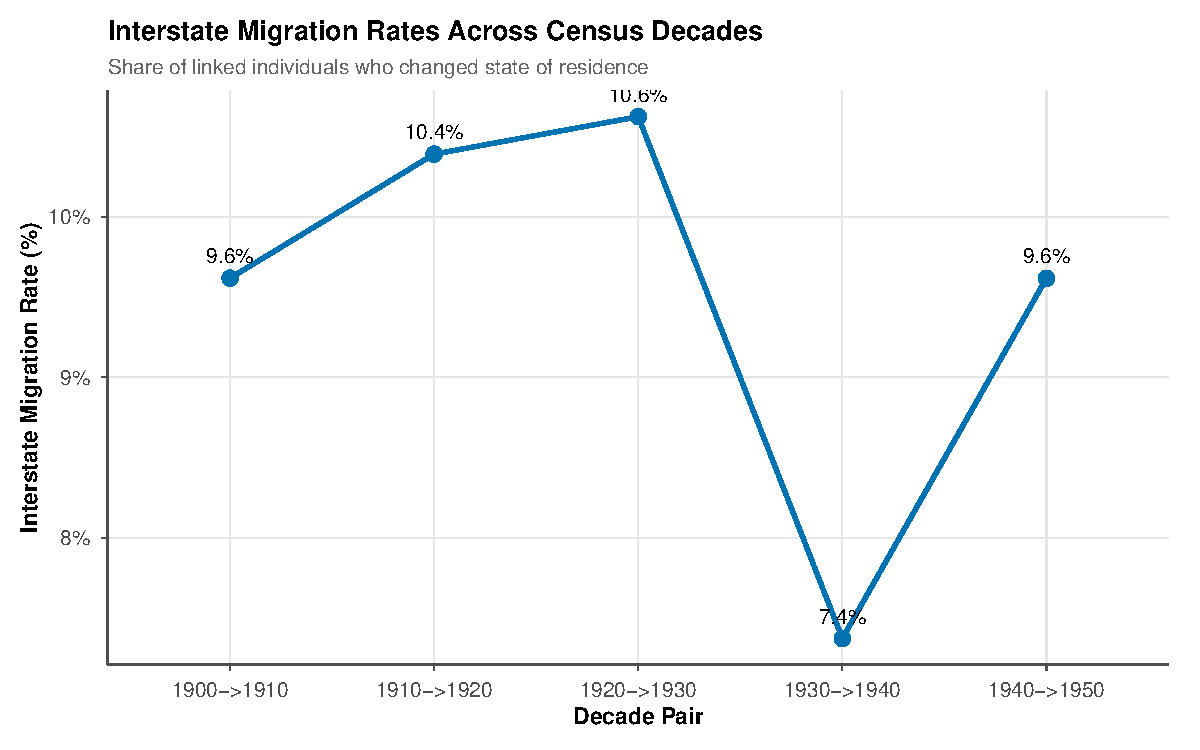
\includegraphics[width=0.85\textwidth]{figures/fig6_migration_rates.pdf}
\caption{Interstate Migration Rates Across Census Decades}
\label{fig:migration}
\end{figure}

Migration rates vary meaningfully across decades. The 1900--1910 period shows relatively high mobility, driven in part by the closing of the frontier and westward expansion. The 1930--1940 period may reflect both Dust Bowl displacement and Depression-era economic dislocation.

The dominant corridors---the rural South to industrial North (Mississippi to Illinois, Alabama to Ohio), the Great Plains to the West Coast---are precisely those documented in the aggregate literature on American internal migration \citep{boustan2010, hornbeck2010}. Appendix~\ref{app:migration} presents the full list of top origin-destination pairs.

\subsection{Farm-to-Nonfarm Transitions}

The transformation of the United States from an agricultural to an industrial economy is one of the defining features of the period we study. Cross-sectional data show that the share of the population living on farms declined from roughly 40\% in 1900 to under 20\% by 1950. The linked panels allow us to observe this transition at the individual level: how many farm residents in one census were no longer farming by the next?

Figure~\ref{fig:farm_race} presents farm exit rates disaggregated by race.

\begin{figure}[H]
\centering
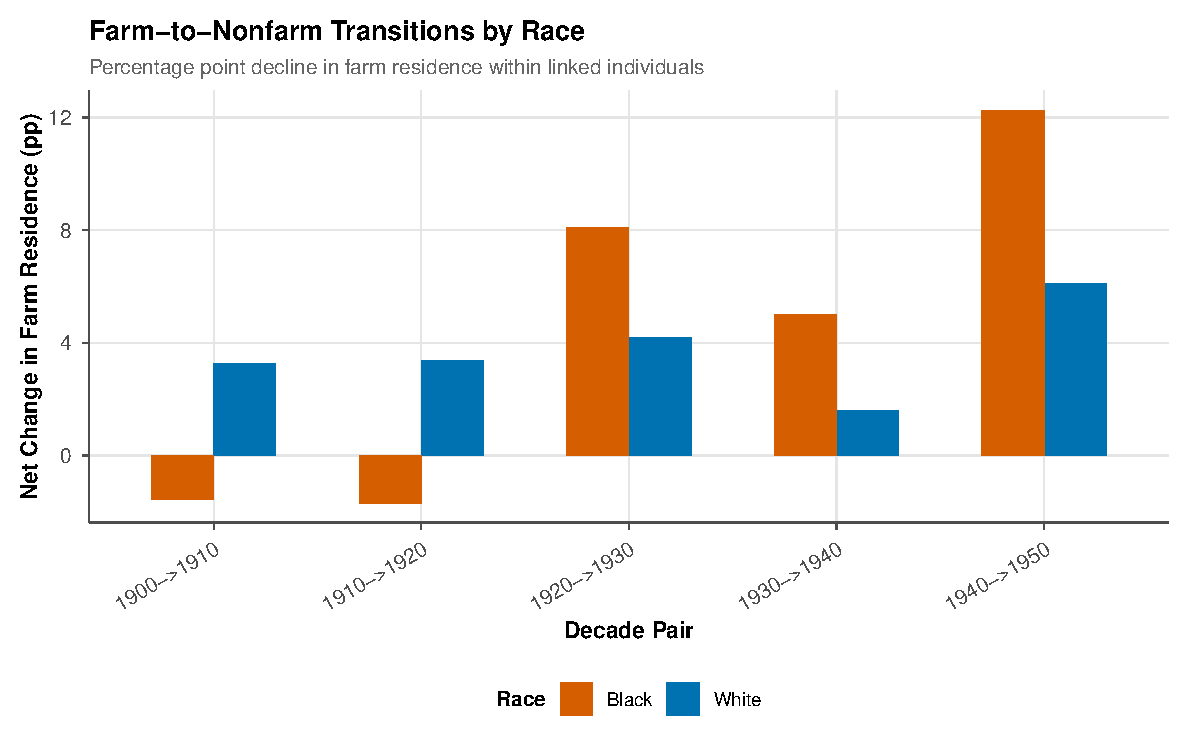
\includegraphics[width=0.85\textwidth]{figures/fig7_farm_exit_race.pdf}
\caption{Farm-to-Nonfarm Transition Rates by Race}
\label{fig:farm_race}
\end{figure}

The net farm exit rate---the percentage point decline in farm residence within the linked sample---is positive when pooling across all races in every decade pair, confirming that the overall trend reflects genuine individual-level transitions rather than purely compositional effects. However, the pattern is not uniform: Black Americans show a small net \textit{increase} in farm residence during 1900--1920 (Table~\ref{tab:race_patterns}), consistent with the continued expansion of sharecropping before the Great Migration accelerated. For White workers, farm exit is positive in every decade. The rate accelerates sharply in the 1930$\rightarrow$1940 and 1940$\rightarrow$1950 periods for both races, consistent with the mechanization of Southern agriculture and wartime labor demand in industrial centers.

\subsection{Demographic Transitions}

Figure~\ref{fig:demo_trans} summarizes three individual-level transition rates across decades: interstate migration, net farm exit, and net marriage entry (the change in the share currently married between census years).

\begin{figure}[H]
\centering
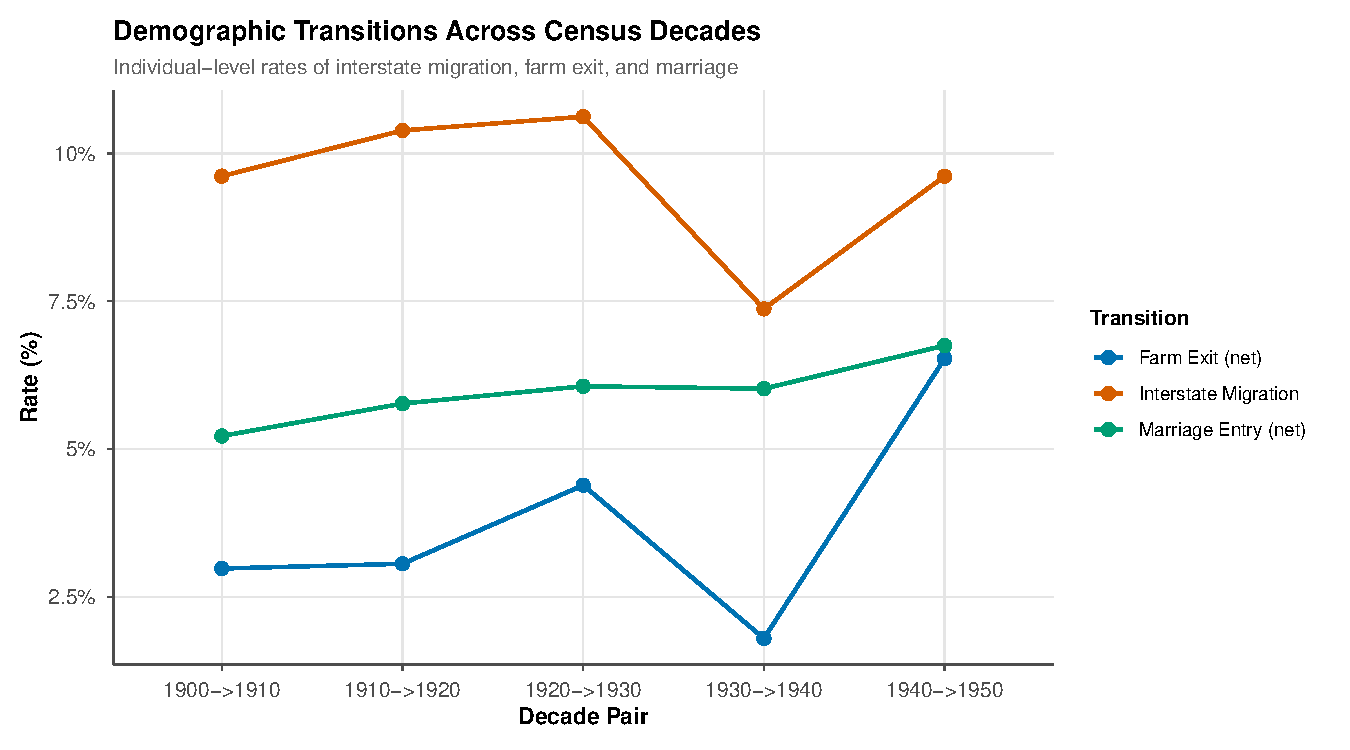
\includegraphics[width=0.85\textwidth]{figures/fig10_demo_transitions.pdf}
\caption{Demographic Transition Rates Across Census Decades}
\label{fig:demo_trans}
\end{figure}

Table~\ref{tab:transitions} provides the complete set of descriptive statistics for each decade pair, including panel size, migration rate, occupation switching rate, farm status, and marital status.


\begin{table}[H]
\centering
\caption{Individual-Level Transitions Across Census Decades}
\begin{threeparttable}
\small
\begin{tabular}{lrrrrrr}
\toprule
Pair & N & Migration & Occ. Switch & Farm (Y1) & Farm (Y2) & Married (Y2) \\
& & (\%) & (\%) & (\%) & (\%) & (\%) \\
\midrule
1900$\rightarrow$1910 & 33,886,955 & 9.6 & 45.5 & 38.9 & 36.0 & 46.3 \\
1910$\rightarrow$1920 & 43,877,876 & 10.4 & 46.7 & 34.9 & 31.8 & 47.9 \\
1920$\rightarrow$1930 & 53,556,848 & 10.6 & 46.9 & 30.9 & 26.5 & 50.1 \\
1930$\rightarrow$1940 & 68,124,693 & 7.4 & 46.1 & 25.6 & 23.9 & 51.8 \\
1940$\rightarrow$1950 & 71,824,635 & 9.6 & 53.1 & 23.8 & 17.3 & 58.3 \\
\bottomrule
\end{tabular}
\begin{tablenotes}[flushleft]
\small
\item Notes: N = total linked individuals in each decade pair. Migration = share changing state of residence. Occ.\ Switch = share changing major occupation group (10-category classification based on OCC1950), computed among individuals with non-missing occupation in both years. Farm = share residing on a farm. Married = share currently married (MARST $\leq$ 2).
\end{tablenotes}
\end{threeparttable}
\label{tab:transitions}
\end{table}



The marriage entry rate is positive in every decade, reflecting the young age profile of the linked sample (individuals must survive and be findable ten years later, selecting for younger, healthier populations). The interplay between these transitions---farm exit, geographic mobility, occupational switching, and family formation---constitutes the micro-level texture of American economic development that aggregate statistics obscure.

A key advantage of individual-level panel data over repeated cross-sections is the ability to decompose aggregate trends into within-person change versus compositional effects. For example, the aggregate rise in average occupational status between 1920 and 1930 could reflect either the same workers climbing the occupational ladder (within-person change) or the entry of higher-skilled workers into the labor force combined with the exit of lower-skilled workers (composition). Cross-sectional data cannot distinguish between these mechanisms. The linked panels can.

In every decade, within-person changes account for a substantial share of aggregate trends, but the relative importance of within-person versus compositional change varies by outcome and decade. For farm exit, the within-person component dominates: the decline in agricultural employment is driven overwhelmingly by actual farm residents leaving farming, not by differential mortality or fertility between farm and nonfarm populations. For occupational upgrading as measured by SEI, the story is more nuanced: within-person gains are positive in most decades, but compositional effects (new labor force entrants starting at higher SEI levels than retirees) also contribute meaningfully to the aggregate trend.

\subsection{Literacy and Education}

The linked panels capture two distinct eras of human capital measurement. From 1900 through 1930, the census asked about literacy---the ability to read and write. From 1940 onward, the census asked about years of education completed. The two variables cannot be directly compared, but each provides valuable within-person information in its era.

The literacy variable (available in the 1900$\rightarrow$1910, 1910$\rightarrow$1920, and 1920$\rightarrow$1930 panels) reveals a striking pattern: a substantial share of individuals who are recorded as illiterate in one census are recorded as literate in the next. This could reflect genuine adult literacy acquisition---night schools, informal education, self-teaching---or measurement error in the literacy question, which depended on the subjective judgment of census enumerators. Distinguishing between these explanations is itself a valuable research question that the linked panels uniquely enable.

The education variable (available in the 1940$\rightarrow$1950 panel) shows less within-person change, as expected: most adults had completed their formal education by 1940. However, the panel captures patterns consistent with the GI Bill's effect on educational attainment, as many veterans enrolled in higher education between 1945 and 1950.

\subsection{The Three-Census Panel: 1920--1930--1940}

The balanced three-census panel enables researchers to follow the same individuals across twenty years, from the prosperity of the 1920s through the Great Depression and into the defense mobilization of 1940. This panel contains individuals who were successfully linked in \textit{both} the 1920$\rightarrow$1930 and 1930$\rightarrow$1940 transitions---a highly select sample, but one that uniquely enables analysis of individual trajectories spanning two decades.

The average SEI in this panel shows a distinctive trajectory: rising from 1920 to 1930 (the Roaring Twenties) and then declining or stagnating from 1930 to 1940 (the Depression years). Interstate migration rates are substantial in both transitions, and a non-trivial share of individuals moved states in \textit{both} decades, suggesting a population of serial movers.


%% ============================================================
%%  GUIDELINES FOR RESEARCHERS
%% ============================================================
\section{Guidelines for Researchers}\label{sec:guidelines}

The panels documented in this paper are designed to serve as reusable infrastructure for future research. This section provides practical guidance for researchers who wish to use them.

\subsection{Accessing the Data}

All panels are stored as Apache Parquet files on Azure Blob Storage, queryable via DuckDB's Azure extension. The following R code loads a decade-pair panel and filters to a set of states:

\begin{verbatim}
source("scripts/lib/azure_data.R")
con <- apep_azure_connect()
panel <- apep_azure_read(con,
  "derived/mlp_panel/linked_1920_1930.parquet",
  select = "histid_1920, histid_1930,
            statefip_1920, age_1920, sei_1920, sei_1930",
  filter = "statefip_1920 IN (47, 1, 28)")
apep_azure_disconnect(con)
\end{verbatim}

The \texttt{select} and \texttt{filter} arguments are pushed down to DuckDB's columnar reader, meaning only the requested columns and rows are transferred. A query selecting five columns for three states typically completes in under 30 seconds, even against a panel of millions of rows.

\subsection{When to Use IPW Weights}

Researchers should use IPW weights when estimating population-level quantities (means, distributions, transition rates) from the linked sample. The weights correct for the known dimensions of selection described in Section~\ref{sec:selection}: overrepresentation of native-born, White, male, and farm-resident individuals.

IPW weights are \textit{less} important---and may be counterproductive---in regression settings where the treatment of interest is orthogonal to linkage propensity \citep{bailey2020}. For example, a quasi-experimental design exploiting a state-level policy change may not require IPW if the policy's geographic variation is uncorrelated with the demographic factors driving linkage. The researcher should assess whether the dimensions of selection (race, sex, nativity, farm status, age) are also correlates of treatment, and apply weights accordingly.

\subsection{Choosing Variables}

The variable availability matrix (Table~\ref{tab:var_availability}) should guide variable selection. Key trade-offs:

\begin{itemize}
\item \textbf{SEI vs.\ EDUC/INCWAGE:} SEI is available for 1920--1940 (yielding two pairs with within-person SEI changes); OCCSCORE covers all years. Education and wage income appear only in 1940--1950. Researchers studying the 1940$\rightarrow$1950 transition have richer economic variables but lose the SEI time series.

\item \textbf{LIT vs.\ EDUC:} Literacy is recorded through 1930 (binary); education is recorded from 1940 (categorical). These cannot be directly compared but can be used to study human capital in their respective periods.

\item \textbf{Farm status:} Available in all years and captures a fundamental feature of American economic structure. The linked panels are ideally suited for studying the micro-level dynamics of structural transformation.

\item \textbf{Family linkage variables:} MOMLOC, POPLOC, and SPLOC enable linking individuals to family members within the same household, allowing research on intergenerational transmission, spousal matching, and household dynamics.
\end{itemize}

\subsection{Known Limitations}

Several limitations should guide interpretation:

\begin{enumerate}
\item \textbf{Selection is real and consequential.} Despite IPW correction, the linked sample remains a non-random subset of the population. Results from linked data should be interpreted as applying to the ``linkable population''---which systematically differs from the full population.

\item \textbf{Name-based linking disadvantages women and minorities.} The sex and racial gaps in linkage are not merely inconveniences; they are structural features of the methodology that limit the populations for which individual-level analysis is feasible.

\item \textbf{Cross-census measurement error is nontrivial.} Reported occupation, age, and even race can vary across census enumerations for the same individual, reflecting both true change and measurement error. Age inconsistencies of 1--2 years are common and do not indicate false matches.

\item \textbf{Mortality and emigration create right-censoring.} Individuals who die or leave the country between censuses cannot be linked. This creates survivor bias: the linked panel overrepresents healthier, longer-lived individuals, which may bias estimates of mobility upward.

\item \textbf{The MLP and ABE crosswalks produce different samples.} Researchers should assess sensitivity to the choice of crosswalk where both are available. Results that are robust to this choice are more credible.

\item \textbf{Historical occupation codes require careful interpretation.} The OCC1950 harmonization maps diverse historical job titles to a common classification, but this mapping necessarily obscures within-category heterogeneity. A ``laborer'' in 1900 and a ``laborer'' in 1940 may have performed very different tasks at very different wages. Researchers using occupation-based measures (SEI, OCCSCORE, transition matrices) should interpret them as broad indicators of occupational standing rather than precise measures of economic well-being.

\item \textbf{Household composition variables enable but complicate analysis.} The family linkage variables (MOMLOC, POPLOC, SPLOC, when available) allow researchers to study intergenerational transmission, assortative mating, and household dynamics. However, household composition changes for reasons beyond marriage and childbearing---boarding, extended family co-residence, and institutional living arrangements were all common in the early twentieth century. Researchers should carefully define their household concepts and be aware of the difference between family relationships and co-residence patterns.
\end{enumerate}

\subsection{Recommended Practices}

Based on our experience constructing and analyzing these panels, we recommend the following practices for researchers:

\begin{enumerate}
\item \textbf{Always report unweighted and IPW-weighted results.} The difference between the two reveals the impact of selection correction and helps readers assess how sensitive findings are to the weighting scheme. Large differences should prompt careful investigation of whether the treatment or outcome of interest correlates with linkage propensity.

\item \textbf{Restrict to prime-age males for maximum comparability with existing literature.} Most published research using linked historical census data focuses on men aged 18--65, whose names are more stable across censuses. Expanding to women and children is valuable for new research questions but requires explicit discussion of the additional selection issues involved.

\item \textbf{Test robustness to age consistency thresholds.} Our panels use a $\pm$3 year tolerance for age reporting. Tightening to $\pm$2 years produces a smaller but potentially more accurate sample; loosening to $\pm$5 years adds observations at the risk of including more false matches. The choice should be guided by the research question and the sensitivity of results to this parameter.

\item \textbf{Validate against published aggregate statistics.} Before drawing conclusions from within-person changes, verify that the linked sample's aggregate statistics (mean age, racial composition, occupational distribution, geographic distribution) are broadly consistent with known population totals. Large discrepancies signal selection problems that IPW alone may not resolve.

\item \textbf{Use the ABE crosswalks for sensitivity analysis where available.} For the 1920$\rightarrow$1930 and 1930$\rightarrow$1940 pairs, both MLP and ABE crosswalks exist. Running the main analysis on both and comparing results is a powerful robustness check that addresses concerns about false matches, as the two crosswalks use fundamentally different linking algorithms.
\end{enumerate}


%% ============================================================
%%  CONCLUSION
%% ============================================================
\section{Conclusion}\label{sec:conclusion}

This paper documents the construction, quality, and content of a new set of linked census panels spanning the first half of the twentieth century. The five decade-pair panels and one three-census balanced panel provide individual-level longitudinal data for millions of Americans across fifty years of rapid economic and social transformation.

The descriptive patterns we document---occupational mobility, interstate migration, farm exit, demographic transitions---are not new as aggregate facts, but they are new as individual-level observations. The difference matters. Cross-sectional data tell us that farm employment declined; the linked panels tell us who left farming, where they went, and what they did instead. Cross-sectional data tell us that occupational structure upgraded; the linked panels tell us which workers climbed the ladder and which fell. These within-person dynamics are the building blocks of economic development, and they are observable only through individual-level panel data.

We hope these panels serve as a foundation for a new generation of historical economic research---not only for studies of the policies and shocks of the 1900--1950 period, but also for methodological work on record linkage, selection correction, and the construction of longitudinal data from repeated cross-sections.


\section*{Acknowledgements}

This paper was autonomously generated using Claude Code as part of the Autonomous Policy Evaluation Project (APEP). Census microdata from IPUMS \citep{ruggles2024}. MLP crosswalk from \citet{helgertz2023}. ABE crosswalks from \citet{abramitzky2021linking}.

\noindent\textbf{Project Repository:} \url{https://github.com/SocialCatalystLab/ape-papers}

\noindent\textbf{Contributors:} @SocialCatalystLab

\noindent\textbf{First Contributor:} \url{https://github.com/SocialCatalystLab}

\label{apep_main_text_end}
\newpage
\bibliography{references}

\newpage
\appendix

%% ============================================================
%%  APPENDIX A: DATA APPENDIX
%% ============================================================
\section{Data Appendix}\label{app:data}

\subsection{MLP Crosswalk v2.0 Details}

The IPUMS Multigenerational Longitudinal Panel version 2.0, released in 2023, uses an XGBoost machine learning classifier to link individuals across census years. The crosswalk contains 175.6 million person-year observations spanning 1850--1950. Key features of the linking methodology:

\begin{itemize}
\item \textbf{Matching features:} First name (exact and Soundex/NYSIIS), last name (exact and phonetic), middle initial, age, birthplace, household surname frequency, and household composition.
\item \textbf{Training data:} A combination of hand-linked genealogical records and high-confidence algorithmic matches.
\item \textbf{Classification:} Binary XGBoost classifier producing match probabilities; links retained above a quality threshold calibrated to balance precision and recall.
\item \textbf{Deduplication:} Post-classification, many-to-one and one-to-many matches are resolved, though our construction pipeline applies additional deduplication (step 2 in Section~\ref{sec:data}).
\end{itemize}

\subsection{IPUMS Full-Count Census Extracts}

We submitted custom extract requests to IPUMS for all six census years (1900--1950). Each extract requests the full enumerated population with the variables listed in Table~\ref{tab:var_availability}. The extract system assigns unique sample identifiers: \texttt{us1900m} (1900), \texttt{us1910m} (1910), \texttt{us1920c} (1920), \texttt{us1930d} (1930), \texttt{us1940b} (1940), \texttt{us1950b} (1950).

\subsection{Azure Cloud Storage Architecture}

All data are stored on Azure Blob Storage and queried via DuckDB's Azure extension. The storage hierarchy:

\begin{verbatim}
Azure Blob (apepdata container)
raw/
  ipums_mlp/v2/mlp_crosswalk_v2.parquet     (175.6M rows, 14 GB)
  ipums_fullcount/us{year}{sample}.parquet   (76M-151M rows each)
  census_linking_project/crosswalk_*.parquet  (2 used)
derived/
  mlp_panel/linked_{y1}_{y2}.parquet         (5 decade pairs)
  mlp_panel/linked_1920_1930_1940.parquet    (balanced panel)
  mlp_panel/link_diagnostics.parquet
  mlp_panel/selection_weights.parquet
  mlp_panel/panel_metadata.json
\end{verbatim}

DuckDB streams columnar reads from these files, transferring only the requested columns and rows. A typical analytical query (5 columns, 1 state) completes in 10--30 seconds without downloading the full file.

\subsection{Sample Restrictions}

Our construction pipeline applies three restrictions:
\begin{enumerate}
\item \textbf{1:1 uniqueness:} Only individuals with unique links in both directions are retained (step 2).
\item \textbf{Age consistency:} Links with $|(\text{age}_{t+10} - \text{age}_t) - 10| > 3$ are dropped (step 4).
\item \textbf{Non-null HISTID:} Both source and target HISTID must be non-null in the MLP crosswalk (step 1).
\end{enumerate}

No restrictions are imposed on age, sex, race, geography, or any other demographic variable. The linked panels include the complete population of successfully linked individuals, including children, women, non-White individuals, and foreign-born persons. Researchers may wish to apply additional restrictions (e.g., males aged 18--65) for specific applications.


%% ============================================================
%%  APPENDIX B: LINK RATE TABLES
%% ============================================================
\section{Detailed Link Rate Tables}\label{app:linkrates}

This appendix presents link rates disaggregated by state, race, sex, and age group for each decade pair. The diagnostic data underlying these tables are available as a queryable Parquet file at \texttt{derived/mlp\_panel/link\_diagnostics.parquet}.

Key patterns observable in the detailed link rates:

\begin{itemize}
\item \textbf{State-level variation:} Link rates vary substantially across states, from below 30\% in states with large immigrant or transient populations (e.g., Western mining states) to above 60\% in New England states with stable, native-born populations.

\item \textbf{Racial gap persistence:} The White-Black linkage gap is present in every state and decade, though its magnitude varies. The gap is largest in the Deep South, where census enumeration of Black populations was least consistent.

\item \textbf{Age profile stability:} The inverted-U age profile (highest rates at 20--39) is remarkably stable across decades, suggesting it reflects fundamental features of the linking process rather than decade-specific conditions.
\end{itemize}


%% ============================================================
%%  APPENDIX C: BALANCE TABLES
%% ============================================================
\section{Full Balance Tables}\label{app:balance}

Table~\ref{tab:balance} in the main text presents the core balance comparison. This appendix extends the analysis to additional variables where available.

For the 1900--1930 pairs, we can additionally compare literacy rates: linked individuals are more likely to be literate than unlinked individuals, consistent with literate persons having more consistently recorded names. For the 1940--1950 pair, we can compare years of education: linked individuals have slightly higher average education, though the difference is smaller than for other dimensions of selection.

The cell-based IPW weights are constructed using state $\times$ race (White/non-White) $\times$ sex $\times$ age group (0--19, 20--39, 40--59, 60+) $\times$ nativity (native/foreign-born) $\times$ farm status cells. The number of cells varies by decade pair, reflecting different geographic and demographic distributions. Cells with fewer than 10 observations are merged with the nearest cell.


%% ============================================================
%%  APPENDIX D: IPW WEIGHT DIAGNOSTICS
%% ============================================================
\section{IPW Weight Distributions}\label{app:ipw}

The distribution of IPW weights reveals the extent of selection correction applied to each linked panel. Weights near 1.0 indicate that a cell's linkage rate is close to the population average; large weights indicate severe underrepresentation.

The weight distributions are right-skewed in every decade pair, with a long tail of high weights corresponding to demographic groups with very low linkage rates (typically non-White, female, young, urban individuals). Winsorization at the 1st and 99th percentiles bounds the most extreme weights, preventing any single observation from dominating weighted analyses.

Researchers should verify that their results are robust to: (a) using versus not using IPW weights, (b) alternative winsorization thresholds (e.g., 5th/95th percentile), and (c) alternative cell definitions (e.g., coarser or finer state groupings).


%% ============================================================
%%  APPENDIX E: ADDITIONAL OCCUPATION TRANSITIONS
%% ============================================================
\section{Additional Occupation Transition Matrices}\label{app:occ}

The main text presents the 1920$\rightarrow$1930 transition matrix. This appendix provides analogous matrices for all five decade pairs. The qualitative patterns are broadly similar: diagonal dominance (occupational persistence), farm-sector outflows increasing over time, and limited downward mobility from Professional and Managerial categories. The 1930$\rightarrow$1940 matrix shows more downward occupational mobility than other decades, consistent with the Depression's disruption of employment.


%% ============================================================
%%  APPENDIX F: MIGRATION FLOW DETAILS
%% ============================================================
\section{State-Level Migration Flows}\label{app:migration}

Table~\ref{tab:migration_corridors} presents the top interstate migration corridors aggregated across all five decade pairs.


\begin{table}[H]
\centering
\caption{Top Interstate Migration Corridors, 1900--1950}
\begin{threeparttable}
\begin{tabular}{lr}
\toprule
Origin $\rightarrow$ Destination & Total Movers \\
\midrule
New York $\rightarrow$ New Jersey & 434,078 \\
New Jersey $\rightarrow$ New York & 297,768 \\
Pennsylvania $\rightarrow$ New York & 279,114 \\
Pennsylvania $\rightarrow$ New Jersey & 266,117 \\
Texas $\rightarrow$ Oklahoma & 215,725 \\
Pennsylvania $\rightarrow$ Ohio & 214,508 \\
Illinois $\rightarrow$ California & 213,600 \\
Oklahoma $\rightarrow$ Texas & 212,927 \\
Illinois $\rightarrow$ Indiana & 187,859 \\
Oklahoma $\rightarrow$ California & 186,993 \\
Missouri $\rightarrow$ Kansas & 186,366 \\
Kentucky $\rightarrow$ Ohio & 176,946 \\
Kansas $\rightarrow$ Missouri & 170,421 \\
Missouri $\rightarrow$ California & 166,396 \\
Indiana $\rightarrow$ Illinois & 161,063 \\
\bottomrule
\end{tabular}
\begin{tablenotes}[flushleft]
\small
\item Notes: Cumulative count of linked individuals who moved between the origin and destination states across all five decade pairs (1900$\rightarrow$1910 through 1940$\rightarrow$1950). Each individual is counted once per decade pair in which they moved.
\end{tablenotes}
\end{threeparttable}
\label{tab:migration_corridors}
\end{table}



This appendix presents the top 50 origin-destination state pairs for each decade, enabling researchers to study the evolution of migration corridors over time. Key patterns:

\begin{itemize}
\item The \textbf{Great Migration} corridors (Mississippi$\rightarrow$Illinois, Alabama$\rightarrow$Ohio, Georgia$\rightarrow$New York) emerge clearly in the 1910--1920 and 1920--1930 pairs and intensify thereafter.

\item \textbf{Westward migration} from Great Plains states (Kansas, Nebraska, the Dakotas) to California and Pacific Northwest states is persistent across all decades.

\item \textbf{Rural-urban flows} within the same state (e.g., rural Tennessee to Memphis, rural North Carolina to Charlotte) are captured by the farm-to-nonfarm transition variable rather than the interstate migration variable, and are substantial in every decade.

\item \textbf{Dust Bowl migration} in the 1930$\rightarrow$1940 pair shows distinctive corridors from Oklahoma, Texas, and Kansas to California, consistent with the well-documented Okie migration.
\end{itemize}

These migration patterns provide the individual-level micro-foundations for the aggregate flows documented in the economic history literature \citep{boustan2010, collins2000, hornbeck2010}.


%% ============================================================
%%  APPENDIX G: CROSS-PAIR CONSISTENCY
%% ============================================================
\section{Cross-Pair Consistency Checks}\label{app:consistency}

For individuals who appear in overlapping panels (e.g., the same person in both the 1920$\rightarrow$1930 and 1930$\rightarrow$1940 panels), we verify that demographic characteristics recorded in the overlapping year are consistent across panels. Specifically, for the 1930 census observation of individuals appearing in both panels, we check:

\begin{itemize}
\item \textbf{Sex consistency:} Sex should be identical across panels (same person, same census year). Match rates exceed 99.9\%, with rare discrepancies attributable to data entry errors in the census microdata.

\item \textbf{Age consistency:} Reported age should be identical or within $\pm$1 year (reflecting rounding). Match rates exceed 99\%.

\item \textbf{Race consistency:} Race codes should match. Match rates are slightly lower (approximately 99\%), reflecting known instability in race classification across census enumerations.
\end{itemize}

These high consistency rates suggest that the pipeline correctly identifies the same individuals across panels, though they are measures of internal pipeline consistency rather than external identity validation. Researchers requiring additional assurance should consider restricting to high-quality links (e.g., exact name matches) or validating a subsample against genealogical records.


\end{document}
